
	
\thiswatermark{\centering \put(-1780,-940){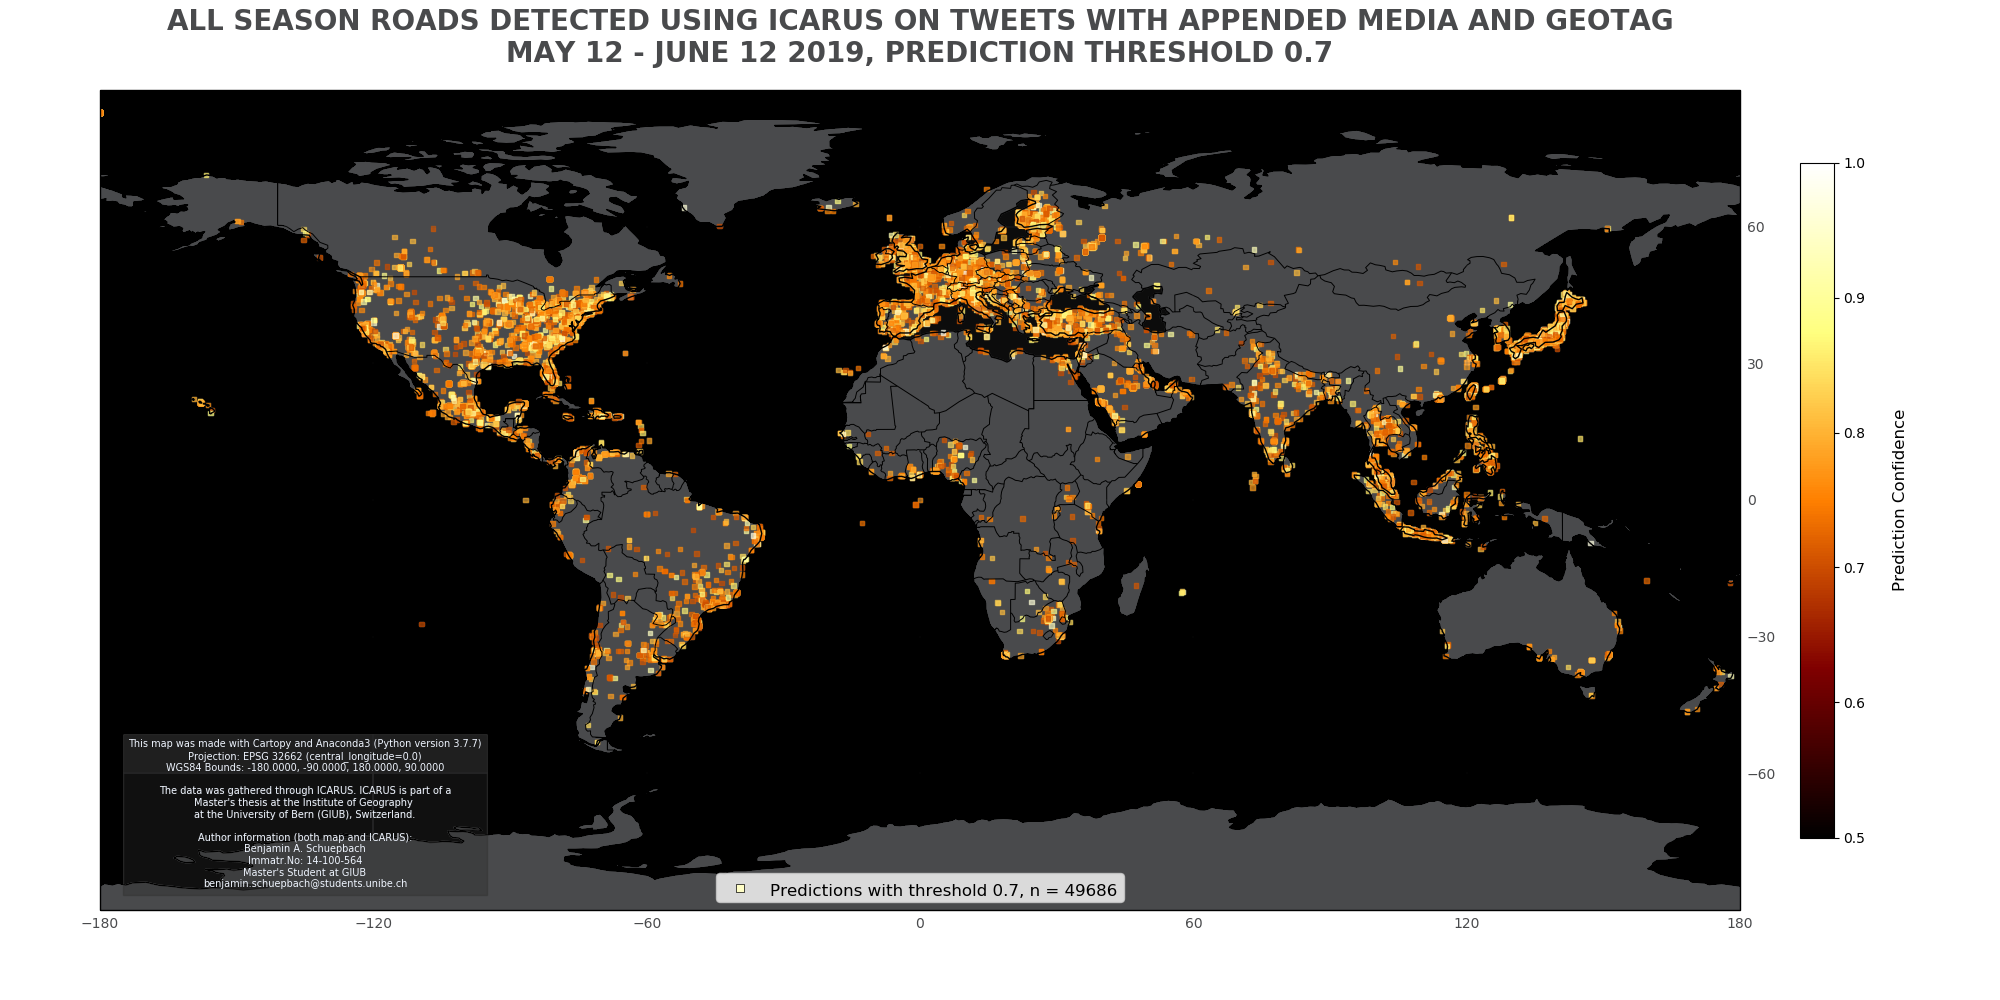
\includegraphics[scale=2]{images/map_ICARUS_thresh70_4.png}} }

\clearpage
\thispagestyle{empty}
\setlength{\hoffset}{-20mm}




\begin{tcolorbox}[standard jigsaw, colback=black, opacityback=1, width=620, opacityframe=0, coltext=white]
	

	{\fontfamily{cmmt}\selectfont{\Huge \textbf{BIGGER IS BETTER. OR IS IT?}}
	
	\bigbreak



		\textbf{{\Large Lessons learned from using a Deep Neural Network on Big Data\\ to estimate SDG Agenda 2030 Target Indicator 9.9.1.}}}



\end{tcolorbox}


\vspace{4cm}

\begin{tcolorbox}[standard jigsaw, colback=black, opacityback=0, width=350, opacityframe=0, coltext=white]
{	
    {\fontfamily{cmmt}\selectfont
	\smallbreak
	
	\Large 
	\textbf{Master's Thesis}
	\bigbreak\bigbreak
	
	\large
	\smallbreak
	Supervision: \bigbreak
	\textbf{PD Dr. Andreas Heinimann\bigbreak}
	Institute of Geography, University of Bern
	\bigbreak
	\bigbreak
	
	
	Author:\bigbreak	
	\textbf{Benjamin Andrea Schüpbach} \bigbreak
	
	Matr.No. 14-100-564
	\smallbreak
	benjamin.schuepbach@students.unibe.ch
	\smallbreak
	Master's Student in Geography
	\smallbreak
	Institute of Geography, University of Bern
	\bigbreak
	

	Bern, XX.XX.2020
	}


}
\end{tcolorbox}


\clearpage
\setlength{\hoffset}{0mm}





\newpage